\documentclass[lettersize,journal]{IEEEtran} % package ieeetran, tlmgr install ieeetran avec TexLive
\usepackage{amsmath,amsfonts}
\usepackage{algorithmic}
\usepackage{algorithm} % package algorithms
\usepackage{array}
\usepackage[caption=false,font=normalsize,labelfont=sf,textfont=sf]{subfig} % package subfig
% On a aussi besoin du package caption
\usepackage{textcomp}
\usepackage{stfloats} % package sttools
\usepackage{url}
\usepackage{verbatim}
\usepackage{graphicx}
\usepackage{cite}
% Aussi besoin de la font pcrr7t qui est dans le package courier
\hyphenation{op-tical net-works semi-conduc-tor IEEE-Xplore}
% updated with editorial comments 8/9/2021

\begin{document}

\title{A Sample Article Using IEEEtran.cls\\ for IEEE Journals and Transactions}

\author{IEEE Publication Technology,~\IEEEmembership{Staff,~IEEE,}
        % <-this % stops a space
\thanks{This paper was produced by the IEEE Publication Technology Group. They are in Piscataway, NJ.}% <-this % stops a space
\thanks{Manuscript received April 19, 2021; revised August 16, 2021.}}

% The paper headers
\markboth{Journal of \LaTeX\ Class Files,~Vol.~14, No.~8, August~2021}%
{Shell \MakeLowercase{\textit{et al.}}: A Sample Article Using IEEEtran.cls for IEEE Journals}

\IEEEpubid{0000--0000/00\$00.00~\copyright~2021 IEEE}
% Remember, if you use this you must call \IEEEpubidadjcol in the second
% column for its text to clear the IEEEpubid mark.

\maketitle

\begin{abstract}
This document describes the most common article elements and how to use the IEEEtran class with \LaTeX \ to produce files that are suitable for submission to the IEEE.  IEEEtran can produce conference, journal, and technical note (correspondence) papers with a suitable choice of class options. 
\end{abstract}

\begin{IEEEkeywords}
Article submission, IEEE, IEEEtran, journal, \LaTeX, paper, template, typesetting.
\end{IEEEkeywords}

\section{Introduction}
\IEEEPARstart{T}{his} file is intended to serve as a ``sample article file''
for IEEE journal papers produced under \LaTeX\ using
IEEEtran.cls version 1.8b and later. The most common elements are covered in the simplified and updated instructions in ``New\_IEEEtran\_how-to.pdf''. For less common elements you can refer back to the original ``IEEEtran\_HOWTO.pdf''. It is assumed that the reader has a basic working knowledge of \LaTeX. Those who are new to \LaTeX \ are encouraged to read Tobias Oetiker's ``The Not So Short Introduction to \LaTeX ,'' available at: \url{http://tug.ctan.org/info/lshort/english/lshort.pdf} which provides an overview of working with \LaTeX.

\section{The Design, Intent, and \\ Limitations of the Templates}
The templates are intended to {\bf{approximate the final look and page length of the articles/papers}}. {\bf{They are NOT intended to be the final produced work that is displayed in print or on IEEEXplore\textsuperscript{\textregistered}}}. They will help to give the authors an approximation of the number of pages that will be in the final version. The structure of the \LaTeX\ files, as designed, enable easy conversion to XML for the composition systems used by the IEEE. The XML files are used to produce the final print/IEEEXplore pdf and then converted to HTML for IEEEXplore.

\section{Where to Get \LaTeX \ Help --- User Groups}
The following online groups are helpful to beginning and experienced \LaTeX\ users. A search through their archives can provide many answers to common questions.
\begin{list}{}{}
\item{\url{http://www.latex-community.org/}} 
\item{\url{https://tex.stackexchange.com/} }
\end{list}

\section{Other Resources}
See \cite{ref1,ref2,ref3,ref4,ref5} for resources on formatting math into text and additional help in working with \LaTeX .

\section{Text}
For some of the remainer of this sample we will use dummy text to fill out paragraphs rather than use live text that may violate a copyright.

Itam, que ipiti sum dem velit la sum et dionet quatibus apitet voloritet audam, qui aliciant voloreicid quaspe volorem ut maximusandit faccum conemporerum aut ellatur, nobis arcimus.
Fugit odi ut pliquia incitium latum que cusapere perit molupta eaquaeria quod ut optatem poreiur? Quiaerr ovitior suntiant litio bearciur?

Onseque sequaes rectur autate minullore nusae nestiberum, sum voluptatio. Et ratem sequiam quaspername nos rem repudandae volum consequis nos eium aut as molupta tectum ulparumquam ut maximillesti consequas quas inctia cum volectinusa porrum unt eius cusaest exeritatur? Nias es enist fugit pa vollum reium essusam nist et pa aceaqui quo elibusdandis deligendus que nullaci lloreri bla que sa coreriam explacc atiumquos simolorpore, non prehendunt lam que occum\cite{ref6} si aut aut maximus eliaeruntia dia sequiamenime natem sendae ipidemp orehend uciisi omnienetus most verum, ommolendi omnimus, est, veni aut ipsa volendelist mo conserum volores estisciis recessi nveles ut poressitatur sitiis ex endi diti volum dolupta aut aut odi as eatquo cullabo remquis toreptum et des accus dolende pores sequas dolores tinust quas expel moditae ne sum quiatis nis endipie nihilis etum fugiae audi dia quiasit quibus.
\IEEEpubidadjcol
Ibus el et quatemo luptatque doluptaest et pe volent rem ipidusa eribus utem venimolorae dera qui acea quam etur aceruptat.
Gias anis doluptaspic tem et aliquis alique inctiuntiur?

Sedigent, si aligend elibuscid ut et ium volo tem eictore pellore ritatus ut ut ullatus in con con pere nos ab ium di tem aliqui od magnit repta volectur suntio. Nam isquiante doluptis essit, ut eos suntionsecto debitiur sum ea ipitiis adipit, oditiore, a dolorerempos aut harum ius, atquat.

Rum rem ditinti sciendunti volupiciendi sequiae nonsect oreniatur, volores sition ressimil inus solut ea volum harumqui to see\eqref{deqn_ex1a} mint aut quat eos explis ad quodi debis deliqui aspel earcius.

\begin{equation}
\label{deqn_ex1a}
x = \sum_{i=0}^{n} 2{i} Q.
\end{equation}

Alis nime volorempera perferi sitio denim repudae pre ducilit atatet volecte ssimillorae dolore, ut pel ipsa nonsequiam in re nus maiost et que dolor sunt eturita tibusanis eatent a aut et dio blaudit reptibu scipitem liquia consequodi od unto ipsae. Et enitia vel et experferum quiat harum sa net faccae dolut voloria nem. Bus ut labo. Ita eum repraer rovitia samendit aut et volupta tecupti busant omni quiae porro que nossimodic temquis anto blacita conse nis am, que ereperum eumquam quaescil imenisci quae magnimos recus ilibeaque cum etum iliate prae parumquatemo blaceaquiam quundia dit apienditem rerit re eici quaes eos sinvers pelecabo. Namendignis as exerupit aut magnim ium illabor roratecte plic tem res apiscipsam et vernat untur a deliquaest que non cus eat ea dolupiducim fugiam volum hil ius dolo eaquis sitis aut landesto quo corerest et auditaquas ditae voloribus, qui optaspis exero cusa am, ut plibus.


\section{Some Common Elements}
\subsection{Sections and Subsections}
Enumeration of section headings is desirable, but not required. When numbered, please be consistent throughout the article, that is, all headings and all levels of section headings in the article should be enumerated. Primary headings are designated with Roman numerals, secondary with capital letters, tertiary with Arabic numbers; and quaternary with lowercase letters. Reference and Acknowledgment headings are unlike all other section headings in text. They are never enumerated. They are simply primary headings without labels, regardless of whether the other headings in the article are enumerated. 

\subsection{Citations to the Bibliography}
The coding for the citations is made with the \LaTeX\ \(\backslash\){\texttt{cite}} command. 
This will display as: see \cite{ref1}.

For multiple citations code as follows: {\texttt{\(\backslash\)cite\{ref1,ref2,ref3\}}}
 which will produce \cite{ref1,ref2,ref3}. For reference ranges that are not consecutive code as {\texttt{\(\backslash\)cite\{ref1,ref2,ref3,ref9\}}} which will produce  \cite{ref1,ref2,ref3,ref9}

\subsection{Lists}
In this section, we will consider three types of lists: simple unnumbered, numbered, and bulleted. There have been many options added to IEEEtran to enhance the creation of lists. If your lists are more complex than those shown below, please refer to the original ``IEEEtran\_HOWTO.pdf'' for additional options.\\

\subsubsection*{\bf A plain  unnumbered list}
\begin{list}{}{}
\item{bare\_jrnl.tex}
\item{bare\_conf.tex}
\item{bare\_jrnl\_compsoc.tex}
\item{bare\_conf\_compsoc.tex}
\item{bare\_jrnl\_comsoc.tex}
\end{list}

\subsubsection*{\bf A simple numbered list}
\begin{enumerate}
\item{bare\_jrnl.tex}
\item{bare\_conf.tex}
\item{bare\_jrnl\_compsoc.tex}
\item{bare\_conf\_compsoc.tex}
\item{bare\_jrnl\_comsoc.tex}
\end{enumerate}

\subsubsection*{\bf A simple bulleted list}
\begin{itemize}
\item{bare\_jrnl.tex}
\item{bare\_conf.tex}
\item{bare\_jrnl\_compsoc.tex}
\item{bare\_conf\_compsoc.tex}
\item{bare\_jrnl\_comsoc.tex}
\end{itemize}





\subsection{Figures}
Fig. 1 is an example of a floating figure using the graphicx package.
 Note that \(\backslash\){\texttt{label}} must occur AFTER (or within) \(\backslash\){\texttt{caption}}.
 For figures, \(\backslash\){\texttt{caption}} should occur after the \(\backslash\){\texttt{includegraphics}}.

\begin{figure}[!t]
\centering
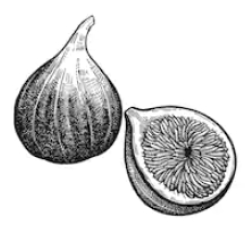
\includegraphics[width=2.5in]{fig1}
\caption{Simulation results for the network.}
\label{fig_1}
\end{figure}

Fig. 2(a) and 2(b) is an example of a double column floating figure using two subfigures.
 (The subfig.sty package must be loaded for this to work.)
 The subfigure \(\backslash\){\texttt{label}} commands are set within each subfloat command,
 and the \(\backslash\){\texttt{label}} for the overall figure must come after \(\backslash\){\texttt{caption}}.
 \(\backslash\){\texttt{hfil}} is used as a separator to get equal spacing.
 The combined width of all the parts of the figure should do not exceed the text width or a line break will occur.
%
\begin{figure*}[!t]
\centering
\subfloat[]{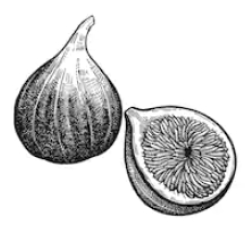
\includegraphics[width=2.5in]{fig1}%
\label{fig_first_case}}
\hfil
\subfloat[]{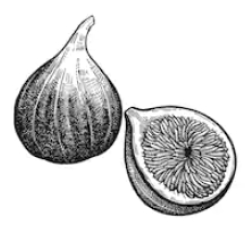
\includegraphics[width=2.5in]{fig1}%
\label{fig_second_case}}
\caption{Dae. Ad quatur autat ut porepel itemoles dolor autem fuga. Bus quia con nessunti as remo di quatus non perum que nimus. (a) Case I. (b) Case II.}
\label{fig_sim}
\end{figure*}

Note that often IEEE papers with multi-part figures do not place the labels within the image itself (using the optional argument to \(\backslash\){\texttt{subfloat}}[]), but instead will
 reference/describe all of them (a), (b), etc., within the main caption.
 Be aware that for subfig.sty to generate the (a), (b), etc., subfigure
 labels, the optional argument to \(\backslash\){\texttt{subfloat}} must be present. If a
 subcaption is not desired, leave its contents blank,
 e.g.,\(\backslash\){\texttt{subfloat}}[].


 

\section{Tables}
Note that, for IEEE-style tables, the
 \(\backslash\){\texttt{caption}} command should come BEFORE the table. Table captions use title case. Articles (a, an, the), coordinating conjunctions (and, but, for, or, nor), and most short prepositions are lowercase unless they are the first or last word. Table text will default to \(\backslash\){\texttt{footnotesize}} as
 the IEEE normally uses this smaller font for tables.
 The \(\backslash\){\texttt{label}} must come after \(\backslash\){\texttt{caption}} as always.
 
\begin{table}[!t]
\caption{An Example of a Table\label{tab:table1}}
\centering
\begin{tabular}{|c||c|}
\hline
One & Two\\
\hline
Three & Four\\
\hline
\end{tabular}
\end{table}

\section{Algorithms}
Algorithms should be numbered and include a short title. They are set off from the text with rules above and below the title and after the last line.

\begin{algorithm}[H]
\caption{Weighted Tanimoto ELM.}\label{alg:alg1}
\begin{algorithmic}
\STATE 
\STATE {\textsc{TRAIN}}\((\mathbf{X} \mathbf{T})\)
\STATE \hspace{0.5cm}\( \textbf{select randomly } W \subset \mathbf{X}  \)
\STATE \hspace{0.5cm}\( N_\mathbf{t} \gets | \{ i : \mathbf{t}_i = \mathbf{t} \} | \) \textbf{ for } \( \mathbf{t}= -1,+1 \)
\STATE \hspace{0.5cm}\( B_i \gets \sqrt{ \textsc{max}(N_{-1},N_{+1}) / N_{\mathbf{t}_i} } \) \textbf{ for } \( i = 1,...,N \)
\STATE \hspace{0.5cm}\( \hat{\mathbf{H}} \gets  B \cdot (\mathbf{X}^T\textbf{W})/( \mathbb{1}\mathbf{X} + \mathbb{1}\textbf{W} - \mathbf{X}^T\textbf{W} ) \)
\STATE \hspace{0.5cm}\( \beta \gets \left ( I/C + \hat{\mathbf{H}}^T\hat{\mathbf{H}} \right )^{-1}(\hat{\mathbf{H}}^T B\cdot \mathbf{T})  \)
\STATE \hspace{0.5cm}\textbf{return}  \(\textbf{W},  \beta \)
\STATE 
\STATE {\textsc{PREDICT}}\((\mathbf{X} )\)
\STATE \hspace{0.5cm}\( \mathbf{H} \gets  (\mathbf{X}^T\textbf{W} )/( \mathbb{1}\mathbf{X}  + \mathbb{1}\textbf{W}- \mathbf{X}^T\textbf{W}  ) \)
\STATE \hspace{0.5cm}\textbf{return}  \(\textsc{sign}( \mathbf{H} \beta )\)
\end{algorithmic}
\label{alg1}
\end{algorithm}

Que sunt eum lam eos si dic to estist, culluptium quid qui nestrum nobis reiumquiatur minimus minctem. Ro moluptat fuga. Itatquiam ut laborpo rersped exceres vollandi repudaerem. Ulparci sunt, qui doluptaquis sumquia ndestiu sapient iorepella sunti veribus. Ro moluptat fuga. Itatquiam ut laborpo rersped exceres vollandi repudaerem. 
\section{Mathematical Typography \\ and Why It Matters}

Typographical conventions for mathematical formulas have been developed to {\bf provide uniformity and clarity of presentation across mathematical texts}. This enables the readers of those texts to both understand the author's ideas and to grasp new concepts quickly. While software such as \LaTeX \ and MathType\textsuperscript{\textregistered} can produce aesthetically pleasing math when used properly, it is also very easy to misuse the software, potentially resulting in incorrect math display.

IEEE aims to provide authors with the proper guidance on mathematical typesetting style and assist them in writing the best possible article. As such, IEEE has assembled a set of examples of good and bad mathematical typesetting \cite{ref1,ref2,ref3,ref4,ref5}. 

Further examples can be found at \url{http://journals.ieeeauthorcenter.ieee.org/wp-content/uploads/sites/7/IEEE-Math-Typesetting-Guide-for-LaTeX-Users.pdf}

\subsection{Display Equations}
The simple display equation example shown below uses the ``equation'' environment. To number the equations, use the \(\backslash\){\texttt{label}} macro to create an identifier for the equation. LaTeX will automatically number the equation for you.
\begin{equation}
\label{deqn_ex1}
x = \sum_{i=0}^{n} 2{i} Q.
\end{equation}

\noindent is coded as follows:
\begin{verbatim}
\begin{equation}
\label{deqn_ex1}
x = \sum_{i=0}^{n} 2{i} Q.
\end{equation}
\end{verbatim}

To reference this equation in the text use the \(\backslash\){\texttt{ref}} macro. 
Please see (\ref{deqn_ex1})\\
\noindent is coded as follows:
\begin{verbatim}
Please see (\ref{deqn_ex1})\end{verbatim}

\subsection{Equation Numbering}
{\bf{Consecutive Numbering:}} Equations within an article are numbered consecutively from the beginning of the
article to the end, i.e., (1), (2), (3), (4), (5), etc. Do not use roman numerals or section numbers for equation numbering.

\noindent {\bf{Appendix Equations:}} The continuation of consecutively numbered equations is best in the Appendix, but numbering
 as (A1), (A2), etc., is permissible.\\

\noindent {\bf{Hyphens and Periods}}: Hyphens and periods should not be used in equation numbers, i.e., use (1a) rather than
(1-a) and (2a) rather than (2.a) for subequations. This should be consistent throughout the article.

\subsection{Multi-Line Equations and Alignment}
Here we show several examples of multi-line equations and proper alignments.

\noindent {\bf{A single equation that must break over multiple lines due to length with no specific alignment.}}
\begin{multline}
\text{The first line of this example}\\
\text{The second line of this example}\\
\text{The third line of this example}
\end{multline}

\noindent is coded as:
\begin{verbatim}
\begin{multline}
\text{The first line of this example}\\
\text{The second line of this example}\\
\text{The third line of this example}
\end{multline}
\end{verbatim}

\noindent {\bf{A single equation with multiple lines aligned at the = signs}}
\begin{align}
a &= c+d \\
b &= e+f
\end{align}
\noindent is coded as:
\begin{verbatim}
\begin{align}
a &= c+d \\
b &= e+f
\end{align}
\end{verbatim}

The {\texttt{align}} environment can align on multiple  points as shown in the following example:
\begin{align}
x &= y & X & =Y & a &=bc\\
x' &= y' & X' &=Y' &a' &=bz
\end{align}
\noindent is coded as:
\begin{verbatim}
\begin{align}
x &= y & X & =Y & a &=bc\\
x' &= y' & X' &=Y' &a' &=bz
\end{align}
\end{verbatim}





\subsection{Subnumbering}
The amsmath package provides a {\texttt{subequations}} environment to facilitate subnumbering. An example:

\begin{subequations}\label{eq:2}
\begin{align}
f&=g \label{eq:2A}\\
f' &=g' \label{eq:2B}\\
\mathcal{L}f &= \mathcal{L}g \label{eq:2c}
\end{align}
\end{subequations}

\noindent is coded as:
\begin{verbatim}
\begin{subequations}\label{eq:2}
\begin{align}
f&=g \label{eq:2A}\\
f' &=g' \label{eq:2B}\\
\mathcal{L}f &= \mathcal{L}g \label{eq:2c}
\end{align}
\end{subequations}

\end{verbatim}

\subsection{Matrices}
There are several useful matrix environments that can save you some keystrokes. See the example coding below and the output.

\noindent {\bf{A simple matrix:}}
\begin{equation}
\begin{matrix}  0 &  1 \\ 
1 &  0 \end{matrix}
\end{equation}
is coded as:
\begin{verbatim}
\begin{equation}
\begin{matrix}  0 &  1 \\ 
1 &  0 \end{matrix}
\end{equation}
\end{verbatim}

\noindent {\bf{A matrix with parenthesis}}
\begin{equation}
\begin{pmatrix} 0 & -i \\
 i &  0 \end{pmatrix}
\end{equation}
is coded as:
\begin{verbatim}
\begin{equation}
\begin{pmatrix} 0 & -i \\
 i &  0 \end{pmatrix}
\end{equation}
\end{verbatim}

\noindent {\bf{A matrix with square brackets}}
\begin{equation}
\begin{bmatrix} 0 & -1 \\ 
1 &  0 \end{bmatrix}
\end{equation}
is coded as:
\begin{verbatim}
\begin{equation}
\begin{bmatrix} 0 & -1 \\ 
1 &  0 \end{bmatrix}
\end{equation}
\end{verbatim}

\noindent {\bf{A matrix with curly braces}}
\begin{equation}
\begin{Bmatrix} 1 &  0 \\ 
0 & -1 \end{Bmatrix}
\end{equation}
is coded as:
\begin{verbatim}
\begin{equation}
\begin{Bmatrix} 1 &  0 \\ 
0 & -1 \end{Bmatrix}
\end{equation}\end{verbatim}

\noindent {\bf{A matrix with single verticals}}
\begin{equation}
\begin{vmatrix} a &  b \\ 
c &  d \end{vmatrix}
\end{equation}
is coded as:
\begin{verbatim}
\begin{equation}
\begin{vmatrix} a &  b \\ 
c &  d \end{vmatrix}
\end{equation}\end{verbatim}

\noindent {\bf{A matrix with double verticals}}
\begin{equation}
\begin{Vmatrix} i &  0 \\ 
0 & -i \end{Vmatrix}
\end{equation}
is coded as:
\begin{verbatim}
\begin{equation}
\begin{Vmatrix} i &  0 \\ 
0 & -i \end{Vmatrix}
\end{equation}\end{verbatim}

\subsection{Arrays}
The {\texttt{array}} environment allows you some options for matrix-like equations. You will have to manually key the fences, but there are other options for alignment of the columns and for setting horizontal and vertical rules. The argument to {\texttt{array}} controls alignment and placement of vertical rules.

A simple array
\begin{equation}
\left(
\begin{array}{cccc}
a+b+c & uv & x-y & 27\\
a+b & u+v & z & 134
\end{array}\right)
\end{equation}
is coded as:
\begin{verbatim}
\begin{equation}
\left(
\begin{array}{cccc}
a+b+c & uv & x-y & 27\\
a+b & u+v & z & 134
\end{array} \right)
\end{equation}
\end{verbatim}

A slight variation on this to better align the numbers in the last column
\begin{equation}
\left(
\begin{array}{cccr}
a+b+c & uv & x-y & 27\\
a+b & u+v & z & 134
\end{array}\right)
\end{equation}
is coded as:
\begin{verbatim}
\begin{equation}
\left(
\begin{array}{cccr}
a+b+c & uv & x-y & 27\\
a+b & u+v & z & 134
\end{array} \right)
\end{equation}
\end{verbatim}

An array with vertical and horizontal rules
\begin{equation}
\left( \begin{array}{c|c|c|r}
a+b+c & uv & x-y & 27\\ \hline
a+b & u+v & z & 134
\end{array}\right)
\end{equation}
is coded as:
\begin{verbatim}
\begin{equation}
\left(
\begin{array}{c|c|c|r}
a+b+c & uv & x-y & 27\\
a+b & u+v & z & 134
\end{array} \right)
\end{equation}
\end{verbatim}
Note the argument now has the pipe "\(\vert\)" included to indicate the placement of the vertical rules.


\subsection{Cases Structures}
Many times cases can be miscoded using the wrong environment, i.e., {\texttt{array}}. Using the {\texttt{cases}} environment will save keystrokes (from not having to type the \(\backslash\){\texttt{left}}\(\backslash\){\texttt{lbrace}}) and automatically provide the correct column alignment.
\begin{equation*}
{z_m(t)} = \begin{cases}
1,&{\text{if}}\ {\beta }_m(t) \\ 
{0,}&{\text{otherwise.}} 
\end{cases}
\end{equation*}
\noindent is coded as follows:
\begin{verbatim}
\begin{equation*}
{z_m(t)} = 
\begin{cases}
1,&{\text{if}}\ {\beta }_m(t),\\ 
{0,}&{\text{otherwise.}} 
\end{cases}
\end{equation*}
\end{verbatim}
\noindent Note that the ``\&'' is used to mark the tabular alignment. This is important to get  proper column alignment. Do not use \(\backslash\){\texttt{quad}} or other fixed spaces to try and align the columns. Also, note the use of the \(\backslash\){\texttt{text}} macro for text elements such as ``if'' and ``otherwise.''

\subsection{Function Formatting in Equations}
Often, there is an easy way to properly format most common functions. Use of the \(\backslash\) in front of the function name will in most cases, provide the correct formatting. When this does not work, the following example provides a solution using the \(\backslash\){\texttt{text}} macro:

\begin{equation*} 
  d_{R}^{KM} = \underset {d_{l}^{KM}} {\text{arg min}} \{ d_{1}^{KM},\ldots,d_{6}^{KM}\}.
\end{equation*}

\noindent is coded as follows:
\begin{verbatim}
\begin{equation*} 
 d_{R}^{KM} = \underset {d_{l}^{KM}} 
 {\text{arg min}} \{ d_{1}^{KM},
 \ldots,d_{6}^{KM}\}.
\end{equation*}
\end{verbatim}

\subsection{ Text Acronyms Inside Equations}
This example shows where the acronym ``MSE" is coded using \(\backslash\){\texttt{text\{\}}} to match how it appears in the text.

\begin{equation*}
 \text{MSE} = \frac {1}{n}\sum _{i=1}^{n}(Y_{i} - \hat {Y_{i}})^{2}
\end{equation*}

\begin{verbatim}
\begin{equation*}
 \text{MSE} = \frac {1}{n}\sum _{i=1}^{n}
(Y_{i} - \hat {Y_{i}})^{2}
\end{equation*}
\end{verbatim}

\section{Conclusion}
The conclusion goes here.


\section*{Acknowledgments}
This should be a simple paragraph before the References to thank those individuals and institutions who have supported your work on this article.



{\appendix[Proof of the Zonklar Equations]
Use \(\backslash\){\texttt{appendix}} if you have a single appendix:
Do not use \(\backslash\){\texttt{section}} anymore after \(\backslash\){\texttt{appendix}}, only \(\backslash\){\texttt{section*}}.
If you have multiple appendixes use \(\backslash\){\texttt{appendices}} then use \(\backslash\){\texttt{section}} to start each appendix.
You must declare a \(\backslash\){\texttt{section}} before using any \(\backslash\){\texttt{subsection}} or using \(\backslash\){\texttt{label}} (\(\backslash\){\texttt{appendices}} by itself
 starts a section numbered zero.)}



%{\appendices
%\section*{Proof of the First Zonklar Equation}
%Appendix one text goes here.
% You can choose not to have a title for an appendix if you want by leaving the argument blank
%\section*{Proof of the Second Zonklar Equation}
%Appendix two text goes here.}



\section{References Section}
You can use a bibliography generated by BibTeX as a .bbl file.
 BibTeX documentation can be easily obtained at:
 http://mirror.ctan.org/biblio/bibtex/contrib/doc/
 The IEEEtran BibTeX style support page is:
 http://www.michaelshell.org/tex/ieeetran/bibtex/
 
 % argument is your BibTeX string definitions and bibliography database(s)
%\bibliography{IEEEabrv,../bib/paper}
%
\section{Simple References}
You can manually copy in the resultant .bbl file and set second argument of \(\backslash\){\texttt{begin}} to the number of references
 (used to reserve space for the reference number labels box).

\begin{thebibliography}{1}
\bibliographystyle{IEEEtran}

\bibitem{ref1}
{\it{Mathematics Into Type}}. American Mathematical Society. [Online]. Available: https://www.ams.org/arc/styleguide/mit-2.pdf

\bibitem{ref2}
T. W. Chaundy, P. R. Barrett and C. Batey, {\it{The Printing of Mathematics}}. London, U.K., Oxford Univ. Press, 1954.

\bibitem{ref3}
F. Mittelbach and M. Goossens, {\it{The \LaTeX Companion}}, 2nd ed. Boston, MA, USA: Pearson, 2004.

\bibitem{ref4}
G. Gr\"atzer, {\it{More Math Into LaTeX}}, New York, NY, USA: Springer, 2007.

\bibitem{ref5}M. Letourneau and J. W. Sharp, {\it{AMS-StyleGuide-online.pdf,}} American Mathematical Society, Providence, RI, USA, [Online]. Available: http://www.ams.org/arc/styleguide/index.html

\bibitem{ref6}
H. Sira-Ramirez, ``On the sliding mode control of nonlinear systems,'' \textit{Syst. Control Lett.}, vol. 19, pp. 303--312, 1992.

\bibitem{ref7}
A. Levant, ``Exact differentiation of signals with unbounded higher derivatives,''  in \textit{Proc. 45th IEEE Conf. Decis.
Control}, San Diego, CA, USA, 2006, pp. 5585--5590. DOI: 10.1109/CDC.2006.377165.

\bibitem{ref8}
M. Fliess, C. Join, and H. Sira-Ramirez, ``Non-linear estimation is easy,'' \textit{Int. J. Model., Ident. Control}, vol. 4, no. 1, pp. 12--27, 2008.

\bibitem{ref9}
R. Ortega, A. Astolfi, G. Bastin, and H. Rodriguez, ``Stabilization of food-chain systems using a port-controlled Hamiltonian description,'' in \textit{Proc. Amer. Control Conf.}, Chicago, IL, USA,
2000, pp. 2245--2249.

\end{thebibliography}


\newpage

\section{Biography Section}
If you have an EPS/PDF photo (graphicx package needed), extra braces are
 needed around the contents of the optional argument to biography to prevent
 the LaTeX parser from getting confused when it sees the complicated
 \(\backslash\){\texttt{includegraphics}} command within an optional argument. (You can create
 your own custom macro containing the \(\backslash\){\texttt{includegraphics}} command to make things
 simpler here.)
 
\vspace{11pt}

\bf{If you include a photo:}\vspace{-33pt}
\begin{IEEEbiography}[{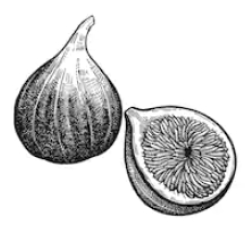
\includegraphics[width=1in,height=1.25in,clip,keepaspectratio]{fig1}}]{Michael Shell}
Use \(\backslash\){\texttt{begin\{IEEEbiography\}}} and then for the 1st argument use \(\backslash\){\texttt{includegraphics}} to declare and link the author photo.
Use the author name as the 3rd argument followed by the biography text.
\end{IEEEbiography}

\vspace{11pt}

\bf{If you will not include a photo:}\vspace{-33pt}
\begin{IEEEbiographynophoto}{John Doe}
Use \(\backslash\){\texttt{begin\{IEEEbiographynophoto\}}} and the author name as the argument followed by the biography text.
\end{IEEEbiographynophoto}




\vfill

\end{document}


